\graphicspath{ {./resources/rob/} }
\documentclass[../templateLTHtwocol.tex]{subfiles}
\begin{document}

Figures \ref{dist_x:fig} - \ref{dist_xyz:fig} compare the performance of the model trained with and without the disturbance. During the evaluation run, the disturbance vector is held constant throughout the episode (step disturbance). The magnitude of the disturbance is varied along with the directions and the expected rewards are recorded individually.

When a disturbance is applied along X or XYZ (figures \ref{dist_x:fig} \& \ref{dist_xyz:fig}), the expected reward appears to increase while applying the disturbance along Z (figure \ref{dist_z:fig}) seems to have a negative impact. A disturbance along XY direction appears to tilt the quadrotor and it appears to leverage the combined effect of the actions taken and the XY component of the wind force, making it approach the hovering point much faster, thus a better reward. This explains why a disturbance along Z has a drastic negative impact, the wind is constantly pushing the quadrotor upwards, and when the magnitude gets large, the quadrotor has to work against the wind. We also observe that the model trained without any disturbance attains a better reward when evaluating disturbances along XY direction. In the case of disturbance along Z, both models seem to perform similarly, and as expected the expected reward decreases with the magnitude of noise, because the agent cannot use the wind force along Z to its advantage, instead it was to work against it.

The robustness evaluation reveals the model trained without any disturbance during the training phase is inherently robust to external disturbances when subjected to wind forces during the testing phase. Not only the model exhibits some form of robustness, but in fact outperforms the model that was subjected to random step disturbances during training. It was also observed that during training injecting a higher magnitude of disturbance resulted in the model not converging, going unstable as expected.
 A plausible explanation is that a single RL agent model is unable to learn/differentiate between the behavior of the combined system, i.e. the drone plus the environment dynamics. Our observations corroborate similar findings reported by a similar study for the cart pole experiment\cite{charac_robustness}. Thus we conclude that training a model subject to external disturbance does not have a significant impact on the model's robustness, but it does help in exploring the environment faster.

Figures \ref{final_x:fig} - \ref{final_xyz:fig} are the simulated 3D trajectories, that show the model stable, reaching the target point $[0,0,1]$. Behavior that is confirmed in hardware with figures \ref{final_hardware:fig} and \ref{hardware:fig}, where the CrazyFlie is subject to disturbances in different directions (wind force exerted manually).



\begin{figure}[H]
	\centering
	\caption{Robustness Evaluation - External Disturbance Injection}
	{Comparing expected rewards of RL policy trained without and with external steps disturbance}
	\begin{subfigure}[b]{0.45\textwidth}
		\caption{Distrubance Along X}
		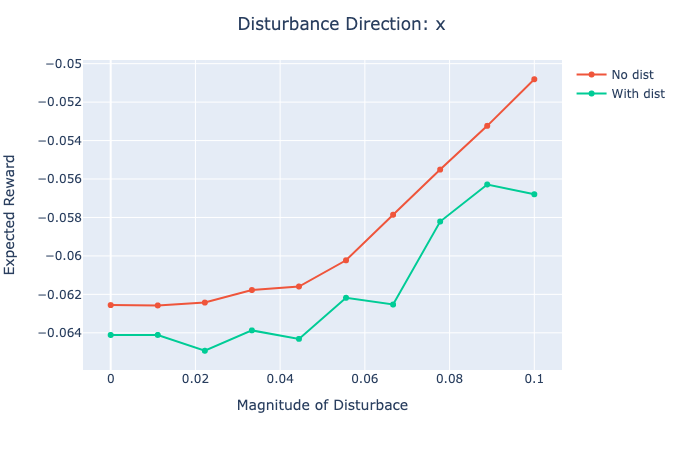
\includegraphics[width=\textwidth]{dist_x.png}
		\label{dist_x:fig}
	\end{subfigure}
	\hfill
	\begin{subfigure}[b]{0.45\textwidth}
		\caption{Distrubance Along Z}
		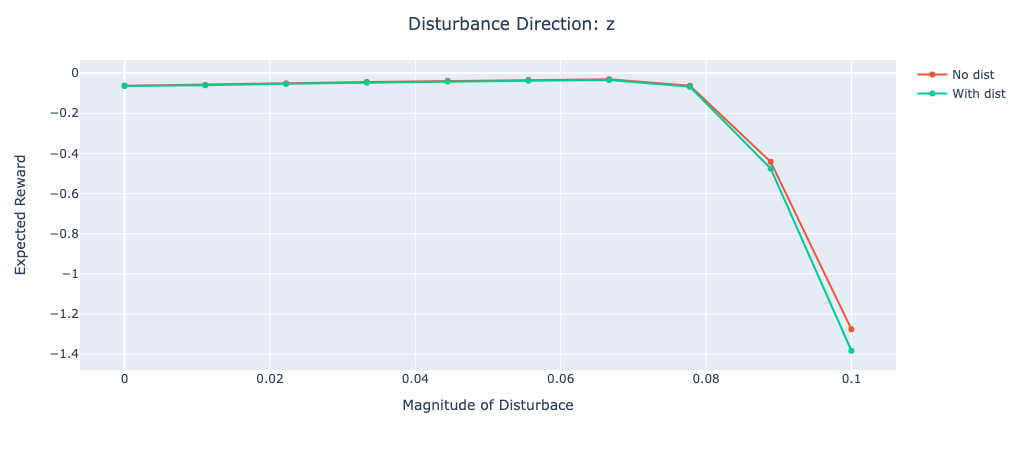
\includegraphics[width=\textwidth]{dist_z.png}
		\label{dist_z:fig}
	\end{subfigure}
	\hfill
	\begin{subfigure}[b]{0.45\textwidth}
		\caption{Distrubance Along XYZ}
		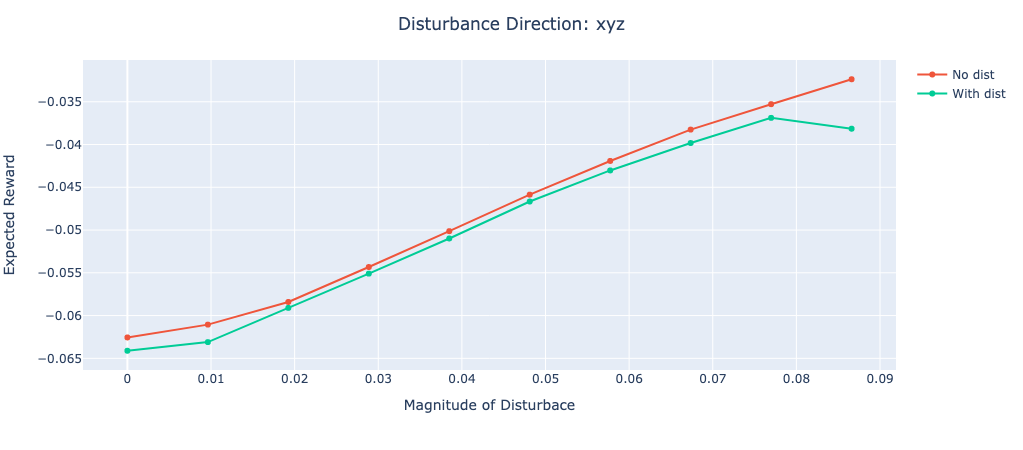
\includegraphics[width=\textwidth]{dist_xyz.png}
		\label{dist_xyz:fig}
	\end{subfigure}
\end{figure}


\begin{figure}[H]
	\centering
	\caption{3D trajectories against disturbances for final model}
	{Robustness against disturbances in simulation and hardware}
	\begin{subfigure}[b]{0.25\textwidth}
		\caption{Distrubance Along X in simulation}
		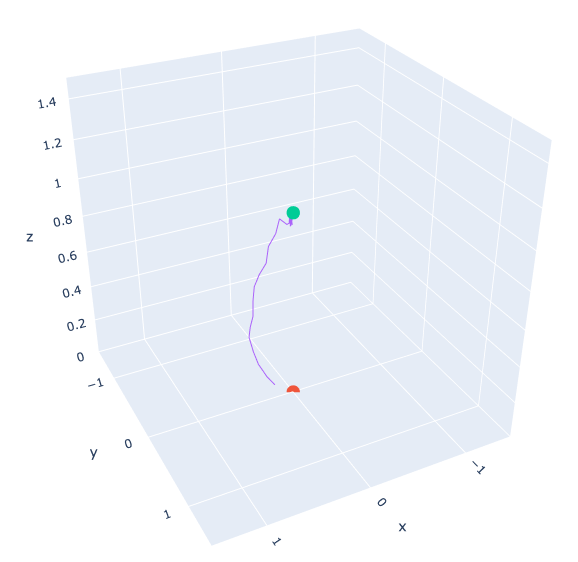
\includegraphics[width=\textwidth]{resources/final_model/3d-dist_x_001.png}
		\label{final_x:fig}
	\end{subfigure}
	\hfill
	\begin{subfigure}[b]{0.25\textwidth}
		\caption{Distrubance Along XYZ in simulation}
		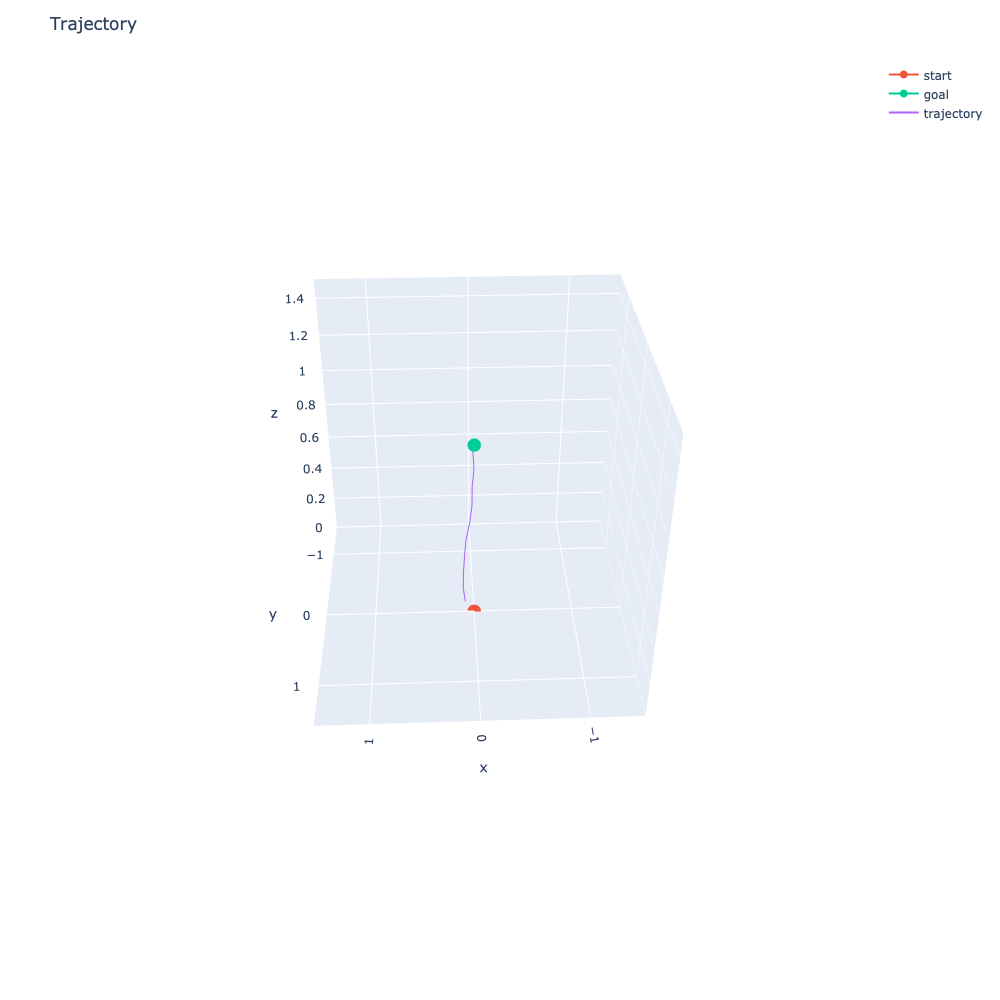
\includegraphics[width=\textwidth]{resources/final_model/3d-dist_xyz_005.png}
		\label{final_xyz:fig}
	\end{subfigure}
	\hfill
	\begin{subfigure}[b]{0.25\textwidth}
		\caption{Distrubances along XYZ on Hardware}
		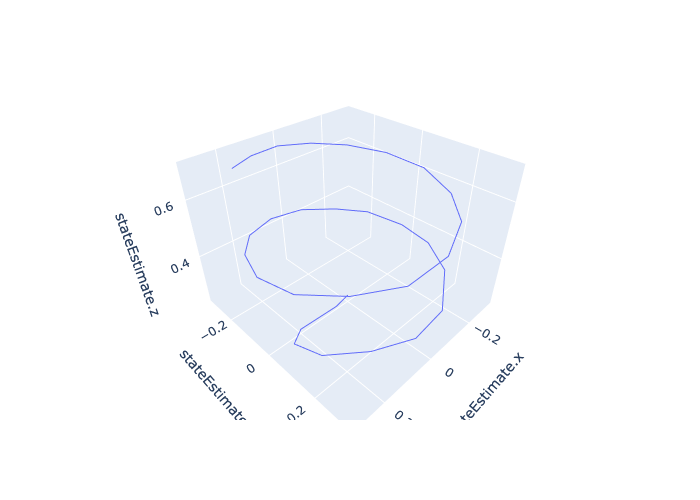
\includegraphics[width=\textwidth]{resources/final_model/3d-trajectory.png}
		\label{final_hardware:fig}
	\end{subfigure}
\end{figure}

\begin{figure}[H]
	\centering
	\caption{Final model hardware test}
	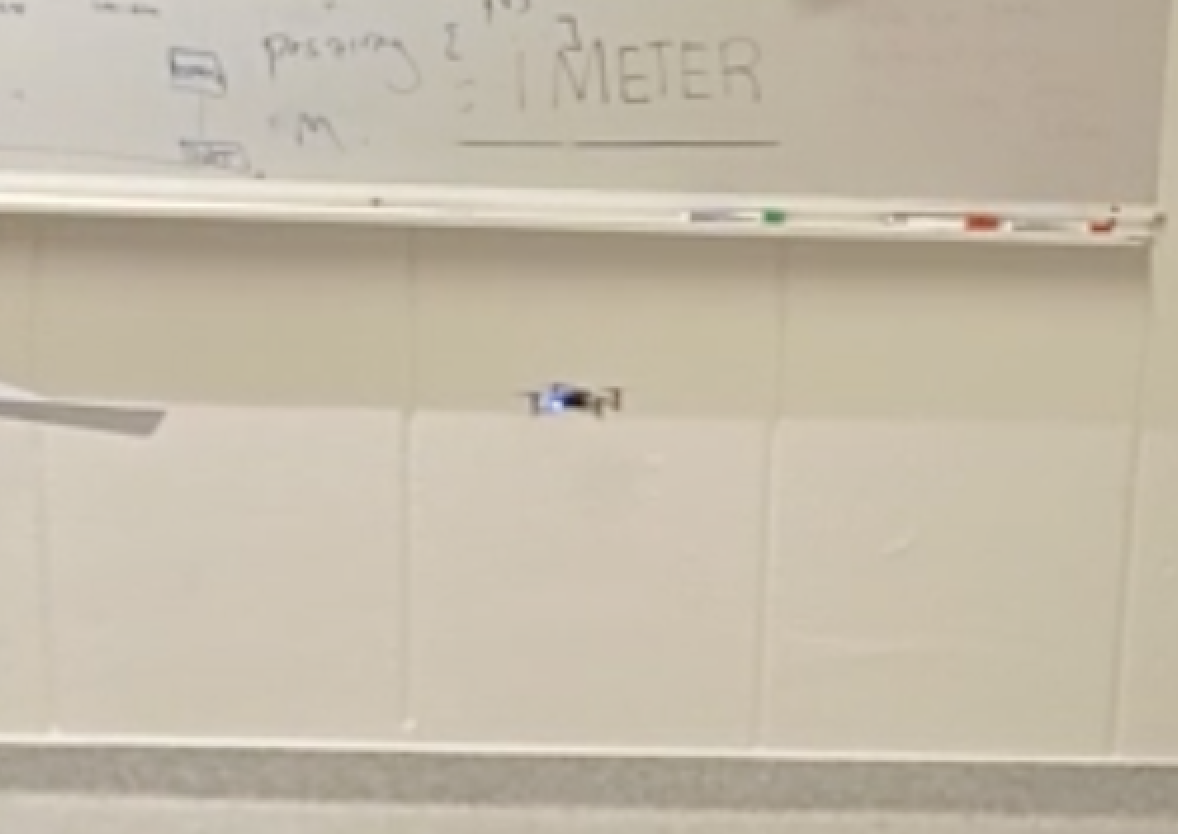
\includegraphics[scale=0.3]{resources/final_model/disturbances_hardware.png}
	\label{hardware:fig}
\end{figure}


\end{document}